\documentclass{article}

%%package
\usepackage{amsmath}
\usepackage{amssymb}
\usepackage{amsthm}
\usepackage{palatino}
\usepackage{tikz}

%% def
\newcommand{\atoms}{\textsf{\small{At}}}
\newcommand{\actions}{\Sigma}
\newcommand{\bisim}[1]{\sim_{#1}}
\newcommand{\mat}[1]{\textbf{Mat}(#1)}
\newcommand{\gs}{\textbf{GS}}


\newcommand{\terms}{T_{K,F_n}}
\newcommand{\universe}{(2^{m})^\gs}
\newcommand{\coproduct}{K \oplus F_n / D}

\newcommand{\todo}[1]{\textbf{TODO:~#1}}

\newtheorem{corollary}{Corollary}
\newtheorem{lemma}{Lemma}

%% main
\begin{document}

\section*{Coalgebraic Decision Procedure for KAT + B!}

%% \subsection*{Motivation}

%% \subsection*{Definitions}
%% The set $\atoms$ are the elements of the boolean algebra B!.
%% The set $K$ is the KAT.
%% The matrices are all of dimension $\atoms \times \atoms$ and contain elements of $K$ in their cells.
%% (In other words, $(\atoms \times \atoms)$-indexed elements of $K$.)

%% This isomorphism is partially made possible by an injection from B! to its language model $2^{\atoms \times \atoms}$.
%% It is $(\atoms \times \atoms)$ because the B! algebra permits tests and assignments.
%% But that's not so important to the current discussion.

%% The language model for KATs is the set of all guarded strings over elements of $K$.
%% Guards are from the embedded boolean algebra of the KAT and strings are from the set of actions $\actions$~of the KAT.

  We want arrows from this diagram and we want $u$ to be unique and $u = I \circ h$.
  \begin{center}
    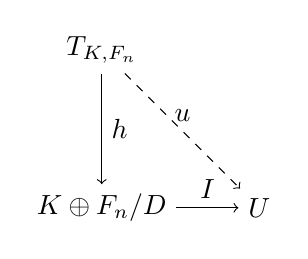
\begin{tikzpicture}
      \node (1) {$\terms$};
      \node [below of=1,yshift=-1cm] (2) {$\coproduct$};
      \node [right of=2,xshift=1cm] (3) {$U$};

      \draw[dashed,->] (1) -- node[above] {$u$} (3);
      \draw[->] (1) -- node[right] {$h$} (2);
      \draw[->] (2) -- node[above] {$I$} (3);
    \end{tikzpicture}
  \end{center}
  
  $\terms$ is the KAT+B!
  
  $\coproduct$ is underlying the algebra of KAT+B!
  

  $U$ is a universe of 0/1 values indexed by first guarded strings and second atoms from the B! algebra.

  (We might be able to simplify the terms $K$ into the pair of sets $(\Sigma,B)$ because we care only about the free KAT.)

  (Can also simplify coproduct to $\mat{2^n, K(\Sigma,B)}$. Now $I$ is an isomorphism.)

\subsection*{Goals}

Want to find an $F X = (2^{2n})^\atoms \times X^{\atoms\actions}$

Need to prove two lemmas:

\begin{lemma}
  $U$ is final F-coalgebra.
  If $L,K \in U$ and $L \bisim{F} K$ then $L = K$.
\end{lemma}
%% \begin{proof}
%% \end{proof}

\begin{lemma}
  The unique F-coalgebra homomorphism satisfies $u = G = I \circ h$
\end{lemma}
%% \begin{proof}
%% \end{proof}

The result of these lemmas is the corollary:
\begin{corollary}
  If $R \subseteq \terms \times \terms$ is an F-bisimulation and $(p,q) \in R$ then KAT+B! $\vDash p = q$
\end{corollary}


\subsection*{h}
The arrow $h : \terms \rightarrow \coproduct$ taking terms from the KAT+B! to matrices representing the commutative coproduct of terms in the KAT and terms in the B! (modulo commutativity conditions) is defined in the original KAT+B! paper as:
\begin{align*}
  h(p)_{\alpha\beta} &= p \hspace{1cm} \mbox{if $\alpha=\beta$}
\\h(0)_{\alpha\beta} &= 0
\\h(1)_{\alpha\beta} &= [\alpha = \beta]
\\h(t?)_{\alpha\beta} &= [\alpha = \beta \le t]
\\h(t!)_{\alpha\beta} &= [\beta = \alpha[t]]
\end{align*}

\subsection*{I}

We define the arrow $I : \coproduct \rightarrow U$ as follows, where $U = (2^{\atoms \times \atoms})^\gs$
\begin{itemize}
\item The commutative coproduct $\coproduct$ is isomorphic to the family of matrices $\mat{\atoms,K}$.
\item There is an injection $\iota$ from any KAT into the language model of KATs: $\iota : KAT \hookrightarrow 2^\gs$.
\item Applying $\iota$ to the entries in the matrices $\mat{\atoms,K}$, gives an injection $\mat{\atoms,K} \hookrightarrow \mat{\atoms,2^\gs}$.
\item By currying, $\mat{\atoms,2^\gs} = (2^{\gs})^{\atoms \times \atoms} = (2^{\atoms \times \atoms})^\gs$.
\end{itemize}

We abbreviate $\atoms \times \atoms$ as $m$, we arrive at a final representation for the universe $U = \universe$.

\subsection*{$I \circ h$}

Let $\hat{\alpha}$ represent an atom of the KAT (to avoid conflicts with the indices $\alpha, \beta$).

\begin{align*}
  I &: \mat{2^n,K} \hookrightarrow \gs \rightarrow 2^n \rightarrow 2
\\
\\I(E(p))(w)_{\alpha\beta} &= [ w \in L(p) ] \hspace{1cm} \mbox{if $\alpha = \beta$}
\\I(h(t?))(\hat{\alpha})_{\alpha\beta} &= [ \alpha = \beta \le t ]
\\I(h(t?))(\hat{\alpha}pw)_{\alpha\beta} &= 0
\\I(A)(w)_{\alpha\beta} &= [ w \in L(A_{\alpha\beta}) ]
\end{align*}

%% \subsubsection*{Bisimilarity}

%% A relations $R \subseteq X \times X$ is an F-bisimulation if for all $(x,y) \in R$, it holds:
%% \begin{enumerate}
%% \item $\varepsilon(x) = \varepsilon(y)$
%% \item $\forall \alpha \in \atoms,~ \rho \in \actions~.~(\delta_{\alpha,\rho}(x), \delta_{\alpha,\rho}(y)) \in R$
%% \end{enumerate}

\subsubsection*{Etc}

%% This diagram is important for the lemmas
\begin{center}
  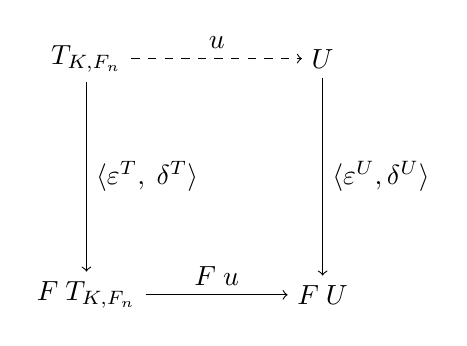
\begin{tikzpicture}
    \node (1) {$\terms$};
    \node[right of=1,xshift=2cm] (2) {$U$};
    \node[below of=1,yshift=-2cm] (3) {$F~T_{K,F_n}$};
    \node[right of=3,xshift=2cm] (4) {$F~U$};

    \draw[dashed,->] (1) -- node[above] {$u$} (2);
    \draw[->] (1) -- node[right] {$\langle \varepsilon^T,~\delta^T\rangle$} (3);
    \draw[->] (2) -- node[right] {$\langle \varepsilon^U,\delta^U \rangle$} (4);
    \draw[->] (3) -- node[above] {$F~u$} (4);
  \end{tikzpicture}
\end{center}

\end{document}
